\section{Introduction}
\label{sec:intro}

Lepton universality is one of the cornerstones of the Standard Model of particle physics. 
In the past years interesting hints of lepton non-universality have been seen in semi-leptonic decays of B hadrons~\cite{HFLAV16} where an excess of $\tau$ final states over $e,\mu$ final states is seen at the level of 4 standard deviations .
Measurements from LEP on W decays also show a hint of non universality at the level of a few percent~\cite{LEP-2}, again with a surplus of $\tau$ final states: 
\begin{equation}
  \label{eq:LEP_BRoverBRAll}
  \frac{2Br(W\to\tau\nu)}{Br(W\to\mu\nu)+Br(W\to e\nu)} = 1.077 \pm 0.026
\end{equation}
resulting in a poor agreement at the level of 2.8 standard deviations, with all correlations included.

Both results are shown in Figure~\ref{fig:lnuhints}.

\begin{figure}[htbp]
\centering
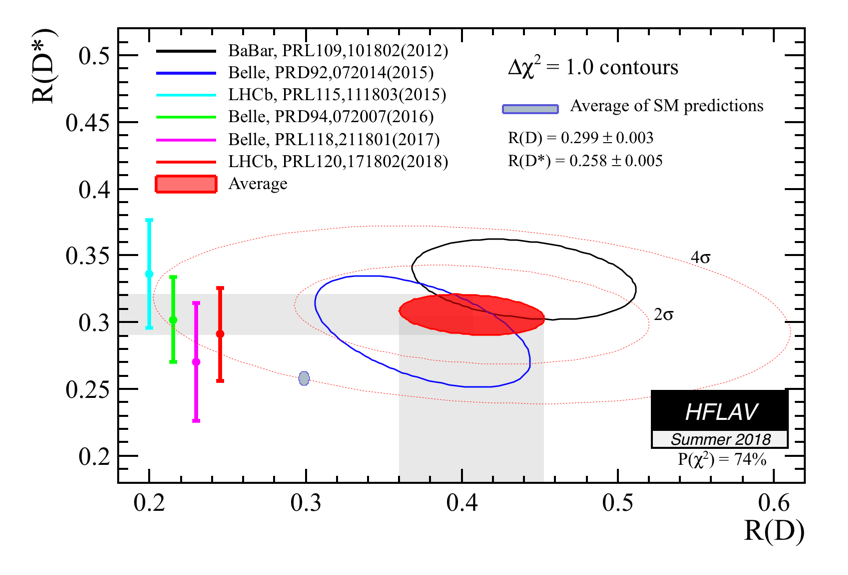
\includegraphics[width=10cm]{figures/rdrds_summer18.png}
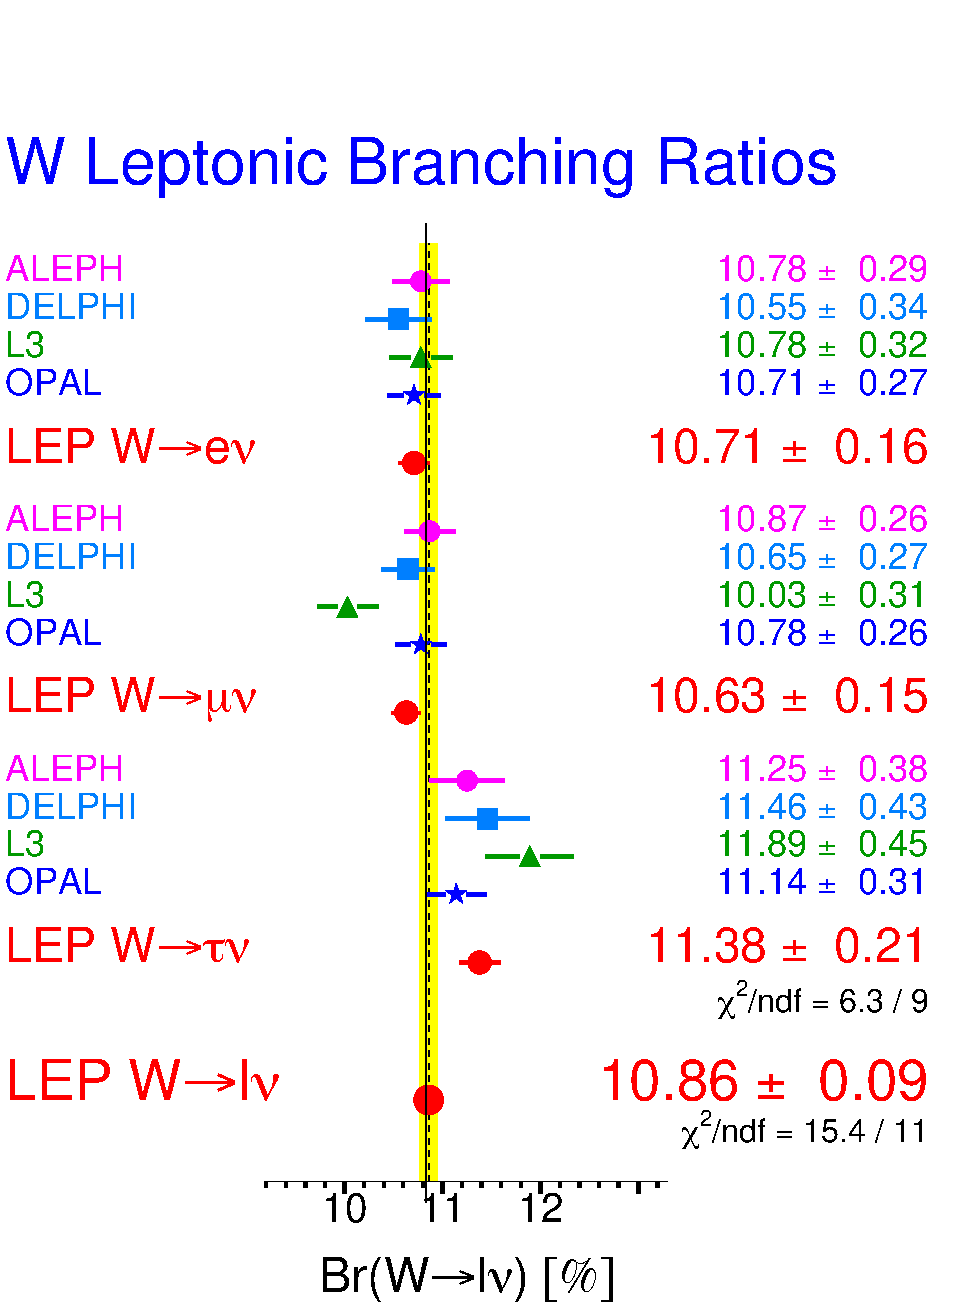
\includegraphics[width=6cm]{figures/4f_brlv_lep_2008.pdf}
\caption{\colorbox{yellow}{Left: Lepton universality in $B\to D^{(*)}$ decay from \cite{HFLAV16}. 
Right:  W leptonic branching ratios from \cite{LEP-2}}}
\label{fig:lnuhints}
\end{figure}

\subsection{Summary of the Analysis Strategy}
The ATLAS experiment has produced over $10^9$ W decays to leptons, which allows us to make a high-precision measurement of lepton (non)-universality in W decay by measuring the ratio $W\rightarrow \tau \rightarrow e/\mu$ / $W \rightarrow e/\mu$ in which many of the systematic effects related to lepton identification cancel. 
Most leptons will come from prompt $W$ decay since the branching fraction of tau to leptons is 17\% and many leptons coming from $W\to\tau\to \ell$ decay do not make it through the L1 trigger because of their lower momentum. 
Our first step will be to identify parts of the phase space enriched in tau decays using a multivariate classifier based on kinematic information and on the impact parameter of the lepton.
Since these to variables are largely uncorrelated we can constrain the efficiency from data.

Control regions are defined to constrain the modelling of the major backgrounds: $Z$ boson production and QCD fake leptons.

